\documentclass[12pt,a4paper]{article}
\usepackage[a4paper,vmargin={1in,1in},hmargin={1.25in,1in}]{geometry}	% Setup of page size,margins
\usepackage{graphics}
\usepackage[font=small,labelfont=bf]{caption}
\usepackage{fancybox}		% For formatting of cover page5
\usepackage{amsmath}    	% For  mathematical formulae
\usepackage{amsfonts}
\usepackage{amssymb}
\usepackage{setspace}		% For adjusting line spacing 
\usepackage{pdfpages}
\usepackage[square, comma, sort&compress,numbers]{natbib} % For customizing citations
\usepackage[pdftex]{hyperref}	% For having working URLs for references 
\usepackage{chngcntr,tocloft}
\counterwithin*{figure}{subsubsection}
\renewcommand{\thefigure}{%
\thesubsubsection.\arabic{figure} %
}
\begin{document}
\pagenumbering{roman}
\pagestyle{empty}
%------------------------------------------------------------------------------
%   Cover Page starts here
%------------------------------------------------------------------------------
\newpage
\pagestyle{empty}
\pagenumbering{gobble}
%\thisfancypage{cmds1}{cmds2}
\thisfancyput(-0.0 in, -10.0 in) {\setlength{\unitlength}{1 in}\framebox(6.7,10.2)}
 
\begin{center}
      
      \textbf{A PROJECT REPORT}\\
      \textbf{ON}
      \vspace{0.2 in}
       
			\end{center}
\vspace{0.1 in}
	\begin{center}
		\textbf{ROVER THERAPIST}\\
	\end{center}
     \vspace{0.2 in}
		\begin{center}
	    SUBMITTED TO THE UNIVERSITY OF PUNE,PUNE \\
	    IN PARTIAL FULFILLMENT OF THE REQUIREMENTS\\
	    FOR THE AWARD OF THE DEGREE 
	\end{center}
	
	\vspace{0.2 in}
	
	\begin{center}
	   \textbf{SUBMITTED BY}
	\end{center}
	\vspace{0.1 in}
	\begin{center}
	\textbf{Shubham Chandak}\\
	\textbf{Ridhima Joshi}\\	
	\textbf{Madhur Lahoti}\\
	\textbf{Radhika Sawant}\\
	\end{center}
	
	\vspace{0.2 in}
	
	\begin{center}
	   \textbf{BACHELOR OF ENGINEERING}\\
	    \begin{small}(B.E Information Technology)
\end{small}	\end{center}

	\vspace{0.2 in}
	
	\begin{center}
	  \textbf{Under the Guidance of}\\
	   \textbf{Prof.C.A.Ghuge}
	\end{center}
		\vspace{0.2 in}
		
		
\begin{center}

\includegraphics[width=2.5cm]{modernlogo}
\end{center}

		\begin{center}
	  \textbf{DEPARTMENT OF INFROMATION TECHNOLOGY}\\
\bf{P.E.S. Modern College of Engineering, } \\
\textbf{Shivaji Nagar, Pune 411 005}\\
\textbf{2014-2015}
	\end{center}
%------------------------------------------------------------------------------
%  Cover ends here
%------------------------------------------------------------------------------

%------------------------------------------------------------------------------
%  Certificate starts here
%------------------------------------------------------------------------------
\newpage
\pagestyle{empty}
 %\thispagestyle{empty}
	\pagenumbering{gobble}
	\thisfancyput(-0.0 in, -10.0 in) {\setlength{\unitlength}{1 in}\framebox(6.7,10.2)}
\begin{center}
\begin{figure}[h]
\centering

\includegraphics[width=2.5 cm]{modernlogo}
\end{figure}
\bf DEPARTMENT OF INFROMATION TECHNOLOGY \\\bf P.E.S Modern College Of Engineering \\
\textbf{Shivajinagar, Pune 411005}
\\
\end{center}
\vspace{0.2in}
\begin{center}
\textbf{\large{C E R T I F I C A T E}}\\
\vspace{0.2in}
\end{center}
		\noindent
  				\setlength{\baselineskip}{1.5\baselineskip}
	\begin{center}
\begin{flushleft}
This is to certify that the following students of Final Year Information Technology have successfully completed the project entitled \textbf{\small"ROVER THERAPIST"}in the academic year 2014-2015.
\end{flushleft} 
\begin{flushleft}
Shubham Chandak\\
Ridhima Joshi\\	
Madhur Lahoti\\
Radhika Sawant\\
\end{flushleft}
\begin{flushleft}
This is partial fulfillment of Bachelor of Information Technology under the University of Pune.
\end{flushleft}
	\end{center} 
		\vspace{0.6 in}
Prof.Mrs.S.D.Deshpande\hspace{0.2 in}  \hspace{2.3 in} Prof.C.A.Ghuge\\
(HOD of Department)\hspace{0.8 in} \hspace{2.0 in}    (Internal Guide)\\\\\\
\singlespace
Place: Pune \hspace{3.5in}  Date:
%------------------------------------------------------------------------------
%  Certificate ends here
%------------------------------------------------------------------------------
%------------------------------------------------------------------------------
%  Acknowledgement starts here
%------------------------------------------------------------------------------
\newpage
\pagenumbering{roman}
\addcontentsline{toc}{section}{ACKNOWLEDGMENT}
\pagestyle{plain}           %For displaying roman page nos
\begin{center}
\bf ACKNOWLEDGEMENT
\end{center}
\hspace{0.7cm}We take this opportunity to thank our project guide Mr. C. A. Ghuge and Head of the Department Prof. Mrs. S. D. Deshpande for their valuable guidance and for providing all the necessary facilities, which were indispensable in the completion of this project report. We are also thankful to all the staff members of the Department of Information Technology of Modern College of Engineering, Pune for their valuable time, support, comments, suggestions and persuasion. We would also like to thank the institute for providing the required facilities, Internet access and important books.  
\begin{flushright}
\hspace{3.5in} 
Shubham Chandak\\
Ridhima Joshi\\	
Madhur Lahoti\\
Radhika Sawant
\end{flushright}

%------------------------------------------------------------------------------
%  Acknowledgement ends here
%------------------------------------------------------------------------------

%------------------------------------------------------------------------------
%  Abstract start here
%------------------------------------------------------------------------------
\newpage
\addcontentsline{toc}{section}{ABSTRACT}
\pagestyle{plain}           %For displaying roman page nos
\begin{center}
\bf ABSTARCT
\end{center}
\hspace{0.7cm} Customer Relationship Management (CRM) is currently one of the most used notions in articles and studies dealing with computer applications. Nowadays it is very difficult for a company to convince a customer (a potential client) with only product or price arguments because of the strong competition in almost all market areas. Aim of our project deals with finding tourist attractions, optimal path finding for tourist attraction, suggestions for way of transportation, seasonal classification, and if the tourist is opting for Rented Vehicle then calculation of the fare using optimal path distance calculation provided by Google Maps API. This project also helps the tourist to lodge a complaint against the Tourist Guide’s, Rented vehicle drivers for diverting the tourist and charging him unfair tariff & finding out emergency numbers for the particular city. Based on the complaint lodged by the passenger the reports are generated and submitted to the higher authorities. Whenever user reaches near to the tourist place images of that place pops up on his phone. Tourist will get the places list as per his location and places are fetched from database as well as Google. Seasonal classification of places is also provided i.e. places to be visited in summer season, winter season and rainy season, this feature will suggest user to visit that particular place which must be visited during that season.

%------------------------------------------------------------------------------
%  Abstarct ends here
%------------------------------------------------------------------------------

%------------------------------------------------------------------------------
%  List of Figures,tables starts here
%------------------------------------------------------------------------------

\newpage
{\setlength{\baselineskip}{1.5\baselineskip}
\listoffigures
\addcontentsline {toc}{section}{LIST OF FIGURES}
}

%------------------------------------------------------------------------------
%  TOC starts here
%------------------------------------------------------------------------------
\newpage
{\setlength{\baselineskip}{1.5\baselineskip}
\tableofcontents
}

%------------------------------------------------------------------------------
%  Introduction start here
%------------------------------------------------------------------------------
\newpage
\pagenumbering{arabic}
\begin{center}
\section{INTRODUCTION}
\end{center}
\pagestyle{plain} 
\hspace{0.7cm}
\\
\subsection{Need}
\begin{itemize}
\item Customer Relationship Management (CRM) is currently one of the most used notions in the articles and studies dealing with computer applications. Nowadays it is very difficult for a company to convince a customer (a potential client) with only product or price arguments because of the strong competition in almost all market areas.
\item Companies therefore reflected how to win the competition. One of the possibilities is to have the better client support – not only in the after sales phase, but also in all other phases of the client communication process, i.e. in the acquisition phase or in the loyalty phase.
\item The grade of customer’s satisfaction is the most relevant factor for the breakdown or the success of a company. Facts such as:
\item One unsatisfied client has a negative influence on up to ten other clients.
\item 60 to 80 percentage of all decisions to buy a certain product are based on the fact that the company offers the better service/client support.
\item One satisfied client positively influences up to three other potential clients.
\item In the long term, five percent of the clients who have a positive image of a company can cause between 25% and 85% new turnover.
\end{itemize}
\\
\subsection{Basic Concept}
\hspace{0.7cm}CRM has been defined in numerous ways and with many descriptions. It can be defined as the art of acquiring customers and having a long-lasting relationship with them. Also, CRM is a combination of people, processes, and technology in order to understand and obtain customers for the company. It focuses on customer retention and builds up the relationship. 
Using CRM, companies can maximize their interactions with customers and obtain a 360-degree vision of customers.CRM is a systematic management of relationships across all parts of the business, focusing on customers, providing long-term value for them, and increasing customer interaction. It also includes communication channels and offers of different services, thereby producing customer retention and loyalty [1].
It is an Android smart phone application, which is built taking into consideration the tourist perspective which guides the tourist to detect his location and get information of nearby places and tourist attractions. It also shows the user the optimal route and helps the user to decide the proper mode of transportation (public or private). If the route is diverted the user gets the alert message and if the user wishes to lodge a complaint against the driver he can do so. The app provides the user the proper tariff according to the distance travelled so that the vehicle driver does not charge unfair tariff.
\\
\subsection{Applications}
\begin{itemize}
\item It is a user friendly application.
\item It helps the tourist to trace the current location and navigate to its destination.
\item As the tourist is new to the city, if the driver tries to divert the route and take the tourist through a longer route an alert message pop’s up saying the route is being diverted.
\item This application guides the tourist to select optimal path.
\item In case, the tourist feels the driver is charging him/her unfair charges he can also lodge a complaint against the driver.
\item Application is also been provided with season wise classification.
\item To help the tourist emergency numbers are also been provided.
\item The tourist can also view the ratings of location and select the place they want to visit accordingly.
\item The image pop up feature is also provided so that the tourist can get the clear view of the location.
\end{itemize}

%------------------------------------------------------------------------------
%  Introduction ends here
%------------------------------------------------------------------------------

%------------------------------------------------------------------------------
%  Literature Survey Satrts here
%------------------------------------------------------------------------------
\newpage
\begin{center}
\section{LITERATURE SURVEY}
\end{center}
\pagestyle{plain} 
\hspace{0.7cm}Literature survey is the most important step in software development process. Before developing the tool it is necessary to determine the time factor, economy n company strength. Once these things are satisfied, ten next steps are to determine which operating system and language can be used for developing the tool. Once the programmers start building the tool the programmers need lot of external support. This support can be obtained from senior programmers, from book or from websites. Before building the system the above consideration are taken into account for developing the proposed system.

\\
\subsection{Customer Relationship Management Using Android Phone in Tourism}
\textbf{Authors:	Nitin Khondre, Ravi Saini, Ronak Jain, 
Sarang Suryawanshi, Bushra Quazi
	Year:		March 2014
Journal: 	International Journal of Emerging Technology and         Advanced Engineering,
	Website: www.ijetae.com (ISSN 2250-2459, ISO 9001:2008 Certified Journal, Volume 4, Issue 3, March 2014)
}
Customers are the vital key for each business and company to help them to grow. So, implementing CRM important tools that will help managers and companies to increase the satisfaction and loyalty of customers more than before. Nowadays it is very difficult for a company to convince a customer with only product or price arguments because of the strong competition in almost all market areas. Mobile technology offers a high potential to significantly transform the ways how a company can interact with their customers and even with own employees. Therefore, this paper deals with the possibilities and aspects to support CRM via future mobile services.
\\

\subsection{inGuide-Interactive Guide}
\textbf{Authors: 	Filipe Andre Gomes Batista, Nuno Rodrigues, and Alexandrino Goncalves
Year: 		2009
Journal:	(2009 3rd IEEE International Conference on Digital Ecosystems and Technologies Future Mobile CRM in Automotive and Tourist Area)
}
This paper describes the inGuide modular application which provides a package management system avoiding the need for a different version of the application for each city. It also describes the geolocation technology in order to provide contextual information in a simple and interactive way. This paper describes two modes those are online mode and offline mode. We preferred online mode of GPS tracking as it gives more accurate location.  
\\

\subsection{On-line GPS Track Simplification Algorithm for Mobile Platforms}
\textbf{Author:	R. Ivanov
	Year:		2010
	Journal:	Information Technology and Control
}

This paper describes an algorithm for on-line simplification of the number of points, describing a GPS track. It is offered on the base of analysis of the location of three last points.
\\

\subsection{Overview on Android- The New Mobile Operating System}
\textbf{Author:	Monika Bazard, Sonia Bhardwaj
	Year:		April, 2011
Journal:	SGI Reflections- International Journal of Science, Technology and             Management. ISSN No. 0976-2140. Volume 2, Issue 1, April, 2011
}

This paper describes the Android’s history, architecture, libraries and its advantages and disadvantages in the smart phones.
\\
%------------------------------------------------------------------------------
%  Literature Survey ends here
%------------------------------------------------------------------------------

%------------------------------------------------------------------------------
%  Algorithm Starts here
%------------------------------------------------------------------------------
\newpage
\begin{center}
\section{ALGORITHM}
\end{center}
\pagestyle{plain}
\subsection{GPS Tracking Algorithim}
\hspace{0.7cm}The data from the GPS receiver are processed by the program module “GPS Provider”. The module “GPS Data Dispatcher” is intended to adaptively define the moment of generation of a new track point. The time interval after which a new point is entered depends on: 
\begin{itemize}
\item Traveled distance
\item The error in the user position  
\item Horizontal accuracy of GPS receiver
\end{itemize}

\begin{figure}[!htb]
\centering
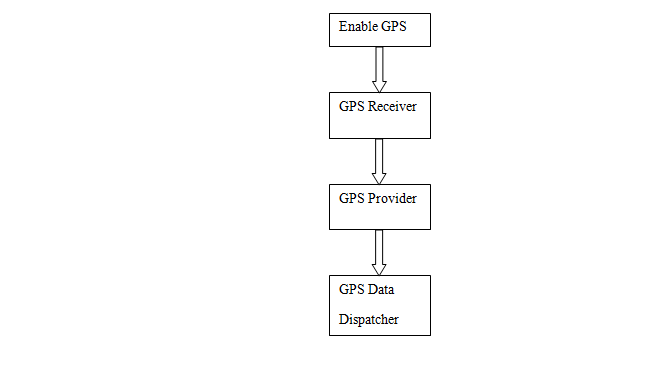
\includegraphics[width=10.5 cm]{point}
\caption{Sequence to obtain the moment to enter a new track point}
\end{figure}

\begin{figure}[!htb]
\centering
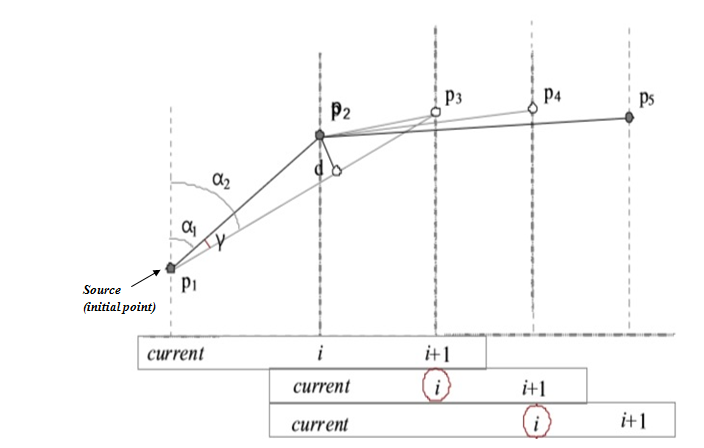
\includegraphics[width=10.5 cm]{track}
\caption{Reduction of the number of points, describing a track}
\end{figure}

\hspace{0.7cm} The proposed tracking algorithm belongs to the distance based algorithms, but the threshold value for the distance after the passing of which a new point is entered is obtained adaptively, taking into account the current accuracy of the user’s position and the travel speed. An additional reduction of the number of points is realized by means of analysis of the position of the last 3 points generated.

The track simplification algorithm that is used belongs to perpendicular distance algorithm.
Point p1 is the last one belonging to the track. Point p2 is the last generated point. It should be defined whether point p2 belongs to the track. For that purpose the value of the angle γ, γ=| α_(1  )-  α_2  |
 The above equation is obtained. If γ≥γ_Th, then it is assumed that point p2 is a part of the track, otherwise point p2 is ignored.

\begin{figure}[!htb]
\centering
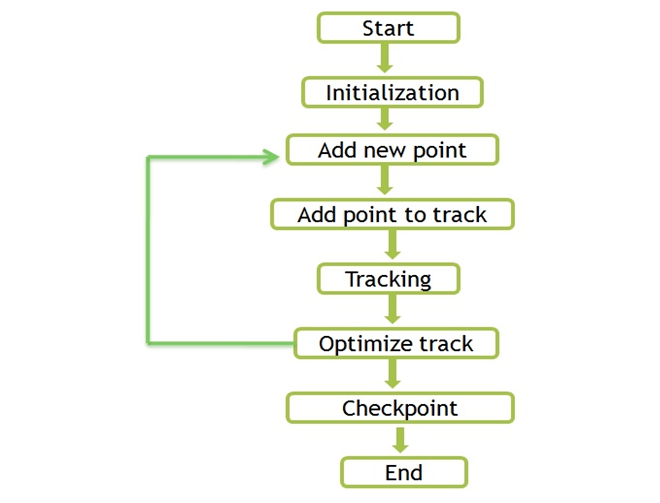
\includegraphics[width=10.5 cm]{flowchart}
\caption{Steps for GPS Tracking}
\end{figure}

\hspace{0.7cm}The module GPS Data Dispatcher is intended to inform through messages the other program modules for events from the GPS receiver. Then the system is initialized and the current point is tracked, it takes the last longitude last latitude and distance threshold after tracking the current point that is the source point the destination point has to be tracked.

	Add new point realizes speed filtering, position filtering, and generation of a new point if there are necessary conditions like HDOP, and the speed and path passed with the needed ranges. After the message is receipted the GPS data is read and the reduction of the points is realized.

	Through the add new pint a new point is inserted and calculated by applying the trigonometric ratios and the shortest distance is traced [2]. 
	
\\
%------------------------------------------------------------------------------
%  ALGORITHM ends here
%------------------------------------------------------------------------------

%------------------------------------------------------------------------------
%  SOFTWARE & HARDWARE REQUIREMENTS starts here
%------------------------------------------------------------------------------
\newpage
\begin{center}
\section{SOFTWARE & HARDWARE REQUIREMENTS}
\end{center}
\pagestyle{plain}
\subsection{HARDWARE & SOFTWARE SPECIFICATIONS}
\subsubsection{HARDWARE INTERFACES}
System requires following hardware interfaces:
\begin{itemize}
\item System		: Intel P4, 2.4 GHZ, 40 GB HDD for installation
\item Memory		: 512 MB memory, 256 MB ram 
\item •	Project’s server side system will be windows based supporting versions windows XP onwards.
\end{itemize}
\subsubsection{SOFTWARE INTERFACES}
\begin{itemize}
\item Eclipse 3.7 Indigo
\item Android SDK
\item Android 2.3
\item Android GPS API
\item Java Standalone HTTP Server
\item Microsoft Access DB
\item UML
\end{itemize}
\subsection{Tools Used}
\subsubsection{Eclipse}
\begin{itemize}
\item Eclipse is an open source community whose projects building tools and frameworks are used for creating general purpose application. The most popular usage of Eclipse is as a Java development environment.
\item Eclipse is an open source community, whose projects are focused on building an open development platform comprised of extensible frameworks, tools and runtimes for building, deploying and managing software across the lifecycle.The Eclipse Foundation is a not-for-profit, member supported corporation that hosts the Eclipse projects and helps cultivate both an open source community and an ecosystem of complementary products and services.
\item In general, the Eclipse Foundation provides four services to the Eclipse community:\\
 1) IT Infrastructure,\\ 
 2) IP Management,\\
 3) Development Process and\\ 
 4) Ecosystem Development.\\
 Full-time staffs are associated with each of these areas and work with the greater Eclipse community to assist in meeting the needs of the stakeholders.
 \end{itemize}
 
\subsubsection{JDK}\\
\begin{itemize}
\item Project Coin support.
\item Editor enhancements: Code completion, hint.
\end{itemize}

\subsubsection{MySQL}\\
\begin{itemize}
\item Simplified connection wizard
\item MySQL 5.0
\item Guided installation to JDBC driver
\item Editing and deployment of stored procedures
\end{itemize}
%------------------------------------------------------------------------------
%  SOFTWARE & HARDWARE REQUIREMENTS ends here
%------------------------------------------------------------------------------

%------------------------------------------------------------------------------
%  DESIGN ends here
%------------------------------------------------------------------------------
\newpage
\begin{center}
\section{DESIGN DIAGRAMS}
\end{center}
\pagestyle{plain}
\subsection{Overview}
\subsubsection{System Initialization} 
\hspace{0.7cm) System gets initialized and detects the current position of the mobile handset of user. 
 
\subsubsection{Listing Tourist Attraction} 
\hspace{0.7cm)The source is detected using the current GPS location and the user is able to see the tourist places and attractions of that particular place/city.  

\subsubsection{Tracking the Path}
\hspace{0.7cm)Once user has selected path, the system will track the path till user reach to the destination. If path is deviated from optimal path, then it will alert user reminding about the divergence. 

\subsubsection{Fare Calculation}
\hspace{0.7cm)Once the destination is reached the exact fare for the journey is calculated based on different parameters stated above. 
 
\subsubsection{Lodge Complaint} 
\hspace{0.7cm)If driver is not agreed with the fare calculated by the system and asking for more Fare, user has the facility to lodge the complaint against the driver. The passenger can fill a small form having the details about him, the driver and his vehicle and the complaint he has against the driver. After filling all these information the user can upload this information to the central database and can send a SMS to higher authorities.  

\subsubsection{Listing the Emergency Numbers} 
\hspace{0.7cm)Based on the GPS location the emergency numbers will be fetched to help the tourist in emergency.  

\begin{figure}[!htb]
\centering
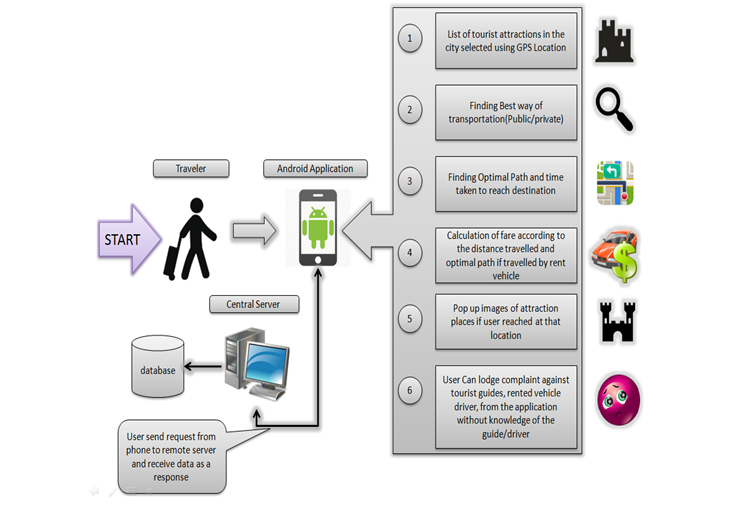
\includegraphics[width=15 cm]{System}
\caption{System Architecture}
\end{figure}
\newpage
\subsection{Data Flow Diagram}
\subsubsection{DFD Level 0}
\begin{figure}[!htb]
\centering
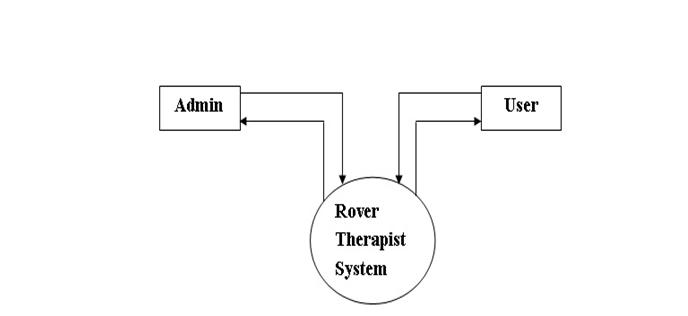
\includegraphics[width=15 cm]{level}
\caption{DFD Level 0}
\end{figure}
\newpage
\subsubsection{DFD Level 1}
\begin{figure}[!htb]
\centering
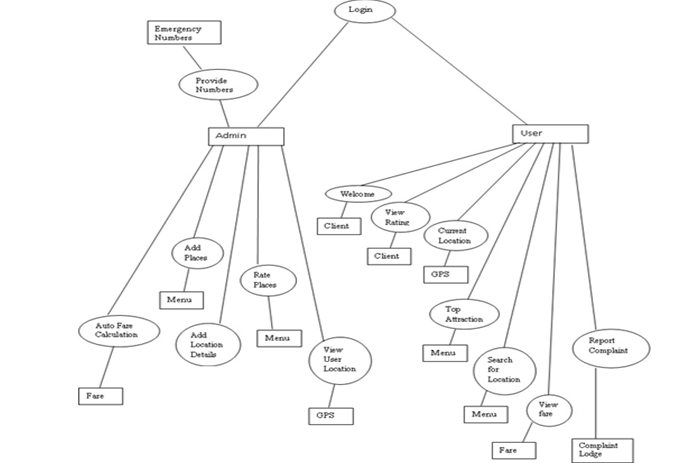
\includegraphics[width=15 cm]{levell}
\caption{DFD Level 1}
\end{figure}
\newpage
\subsection{ER Diagram}
\begin{figure}[!htb]
\centering
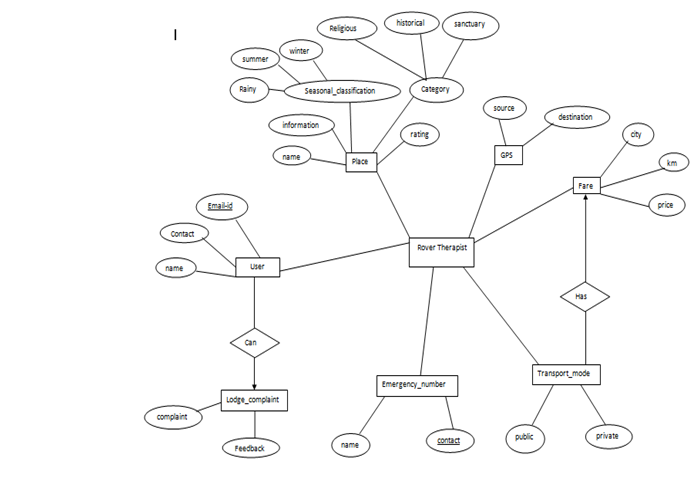
\includegraphics[width=12 cm]{er}
\caption{ER Diagram}
\end{figure}
\newpage
\subsection{UML Diagrams}
\subsubsection{Use Case Diagram}
\begin{figure}[!htb]
\centering
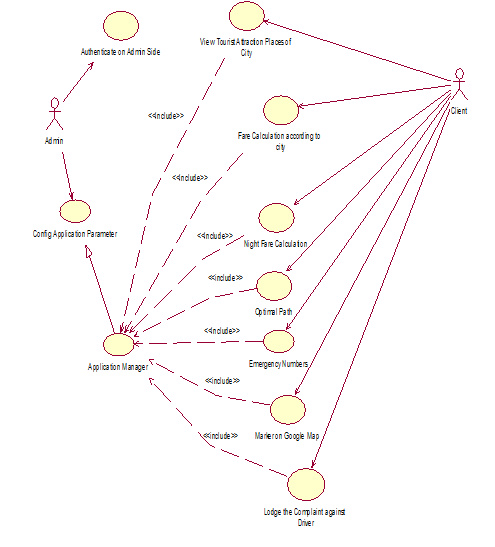
\includegraphics[width=15 cm]{UseCase}
\caption{Use Case Diagram}
\end{figure}
\newpage
\subsubsection{Class Diagram}
\begin{figure}[!htb]
\centering
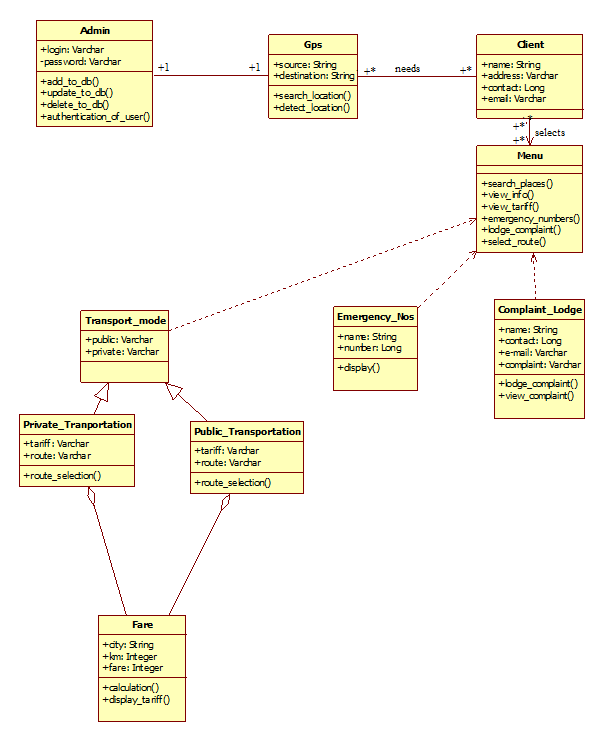
\includegraphics[width=15 cm]{class}
\caption{Class Diagram}
\end{figure}
\newpage
\subsubsection{Activity Diagram}
\begin{figure}[!htb]
\centering
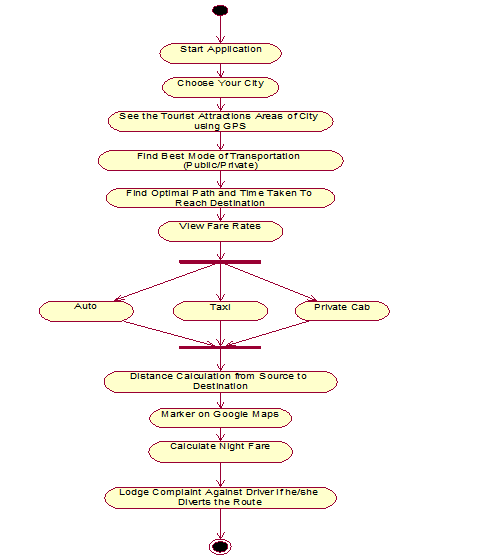
\includegraphics[width=15 cm]{activity}
\caption{Activity Diagram}
\end{figure}
\newpage
\subsubsection{Package Diagram}
\begin{figure}[!htb]
\centering
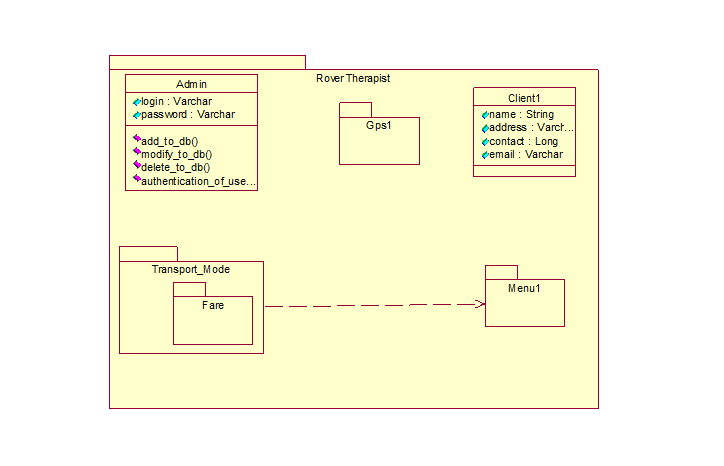
\includegraphics[width=15 cm]{package}
\caption{Package Diagram}
\end{figure}
\newpage
\subsubsection{Sequence Diagram}
\begin{figure}[!htb]
\centering
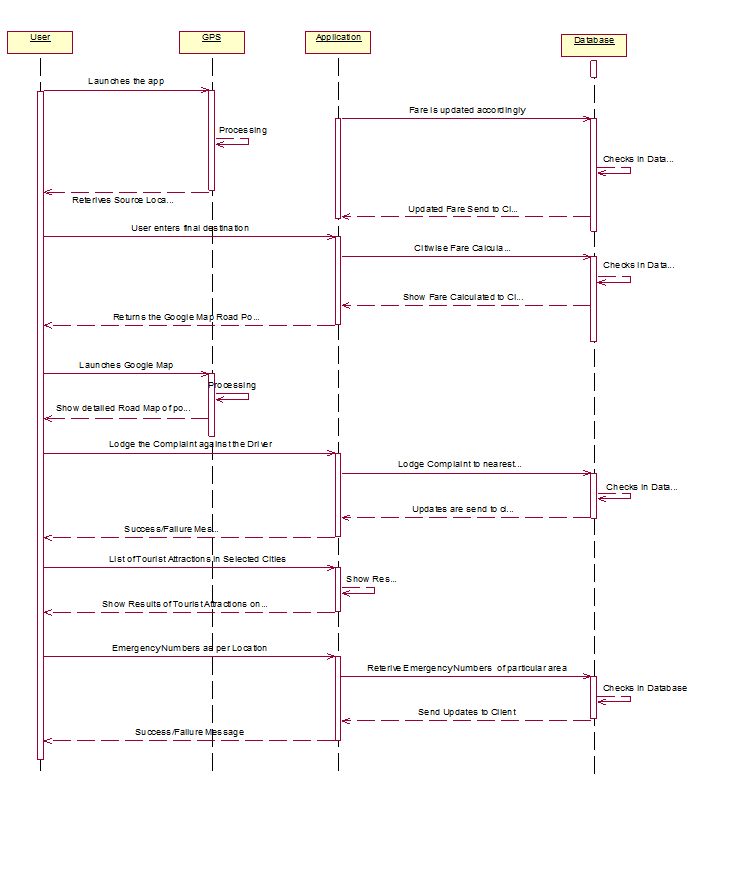
\includegraphics[width=15 cm]{Seq}
\caption{Sequence Diagram}
\end{figure}
\newpage
\subsubsection{Communication Diagram}
\begin{figure}[!htb]
\centering
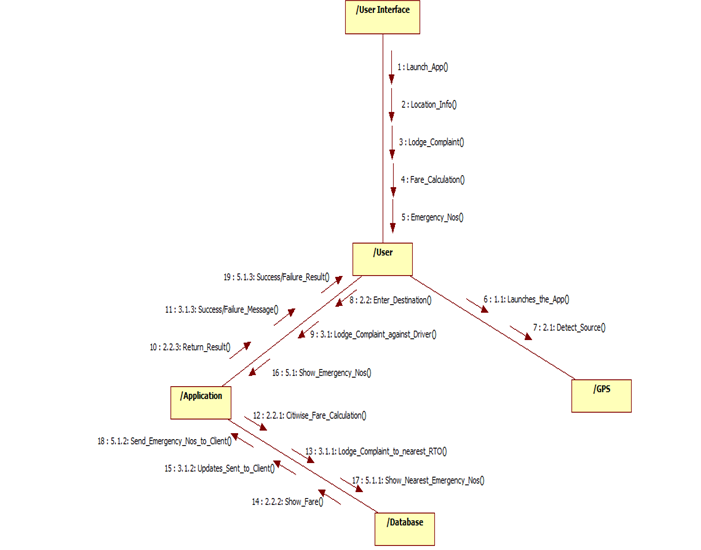
\includegraphics[width=15 cm]{communication}
\caption{Communication Diagram}
\end{figure}
\newpage
\subsubsection{Composite Structure Diagram}
\begin{figure}[!htb]
\centering
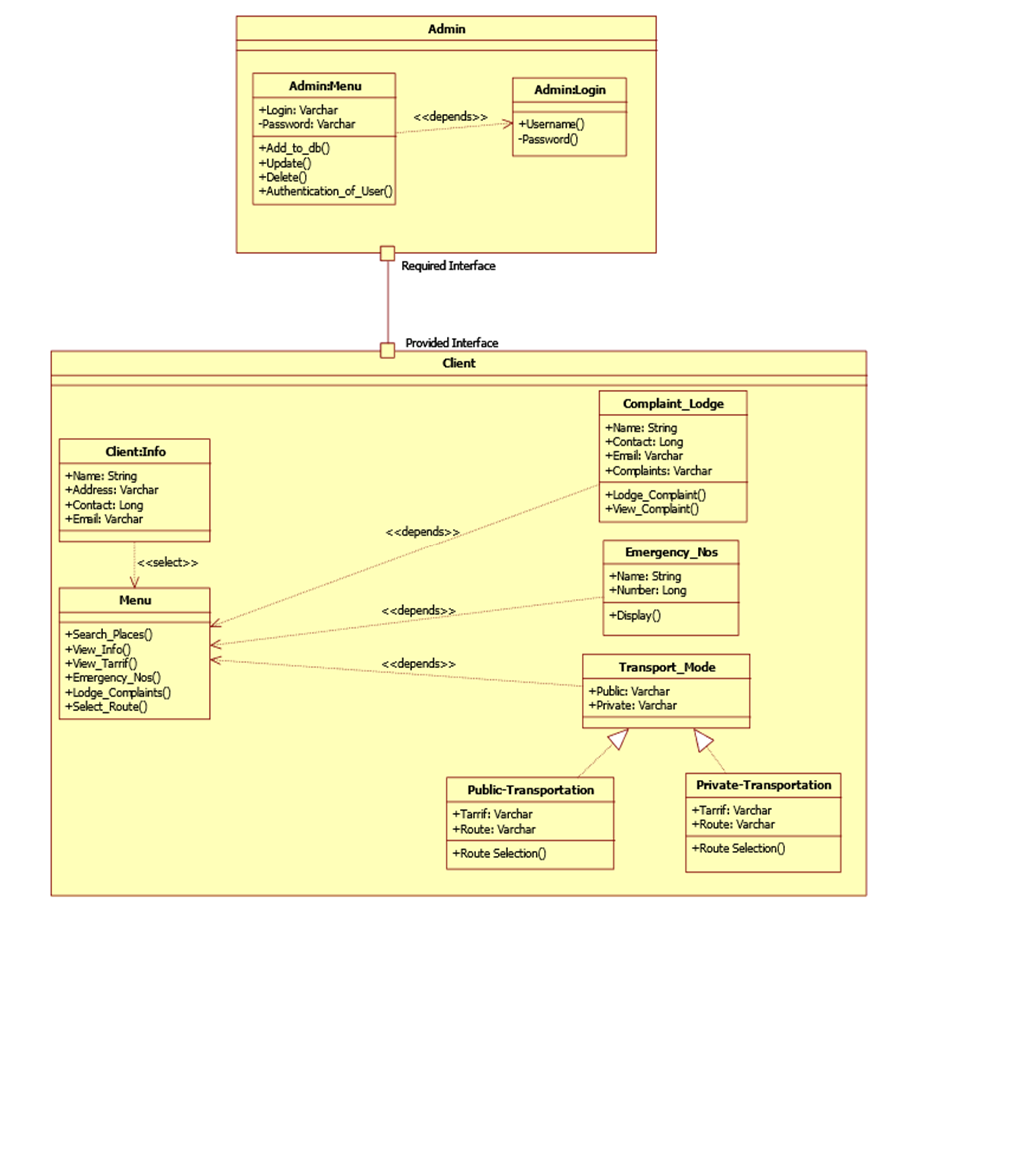
\includegraphics[width=15 cm]{composite}
\caption{Composite Structure Diagram}
\end{figure}
\newpage
\subsubsection{State Machine Diagram}
\begin{figure}[!htb]
\centering
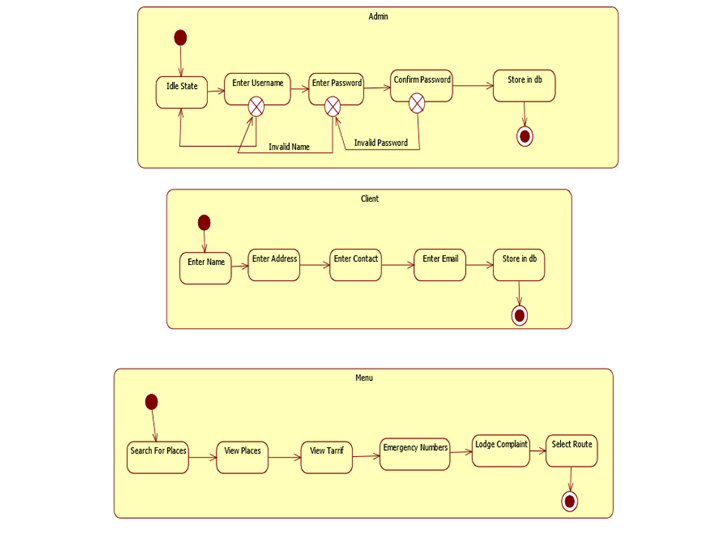
\includegraphics[width=15 cm]{state}
\caption{State Machine Diagram}
\end{figure}
\newpage
\subsubsection{Component Diagram}
\begin{figure}[!htb]
\centering
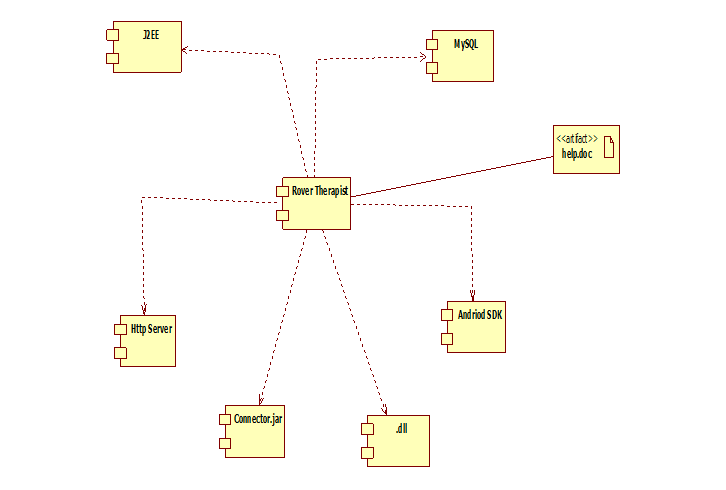
\includegraphics[width=15 cm]{component}
\caption{Component Diagram}
\end{figure}
\newpage
\subsubsection{Deployment Diagram}
\begin{figure}[!htb]
\centering
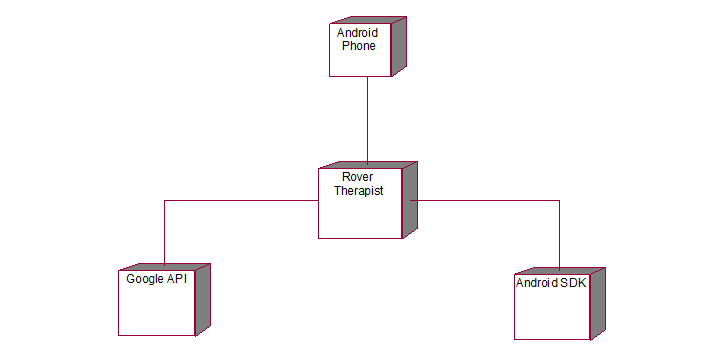
\includegraphics[width=15 cm]{deployment}
\caption{Deployment Diagram}
\end{figure}
%------------------------------------------------------------------------------
%  DESIGN ends here
%------------------------------------------------------------------------------

%------------------------------------------------------------------------------
%  Refernce Starts here
%------------------------------------------------------------------------------
\newpage
\begin{center}
\section{REFRENCES}
\end{center}
\pagestyle{plain}
\begin{enumerate}
\item Nitin Khondre, Ravi Saini, Ronak Jain, Sarang Suryawanshi, Bushra Quazi, Customer   Relationship Management Using Android Phone in Tourism, International Journal of Emerging Technology and Advanced Engineering.

\item R. Ivanov On-line GPS Track Simplification Algorithm for Mobile Platforms, Information Technology and control, 2010.

\item Filipe Andre Gomes Batista, Nuno Rodrigues, and Alexandrino Goncalves, inGuide-Interactive Guide, 2009 3rd IEEE International Conference on Digital Ecosystems and Technologies Future Mobile CRM in Automotive and Tourist Area.

\item Monika Bazard, Sonia Bhardwaj, Overview on Android- The New Mobile Operating System, International Journal of Science, Technology and Management Volume 2, Issue 1, April, 2011.

\item www.javatpoint.com

\item www.develpoer.android.com

\end{enumerate}
%------------------------------------------------------------------------------
%  Refernce ends here
%------------------------------------------------------------------------------
\end{document}

